\section{Analysis}

To help reduce noise, the two traces in each data set were averaged. 
Then, I did boxcar smoothing on the averaged values, which replaces each data point with the average of nearby values, as shown in Equation~\ref{eq:boxcar}. 

\begin{equation}
Y_k = \frac{1}{2r + 1} \sum_{m=-r} y_k+m
\label{eq:boxcar}
\end{equation}

$r$ determines the number of neighboring points included in the average. In this analysis, I used $r = 3$ because it provided the best
results for my figures.

After boxcar smoothing, the peak value of the signal was identified and compared to the background noise. 
This was done with the signal to noise ratio, defined in Equation~\ref{eq:snr}.
\begin{equation}
\mathrm{SNR} = \frac{S_{\mathrm{peak}} - \mu_{\mathrm{noise}}}{\sigma_{\mathrm{noise}}}
\label{eq:snr}
\end{equation}

\subsection{Cassiopeia A}

These are the two Cassiopeia A data sets with averaging and smoothing methods as described above.

\begin{figure}[h!]
\begin{center}
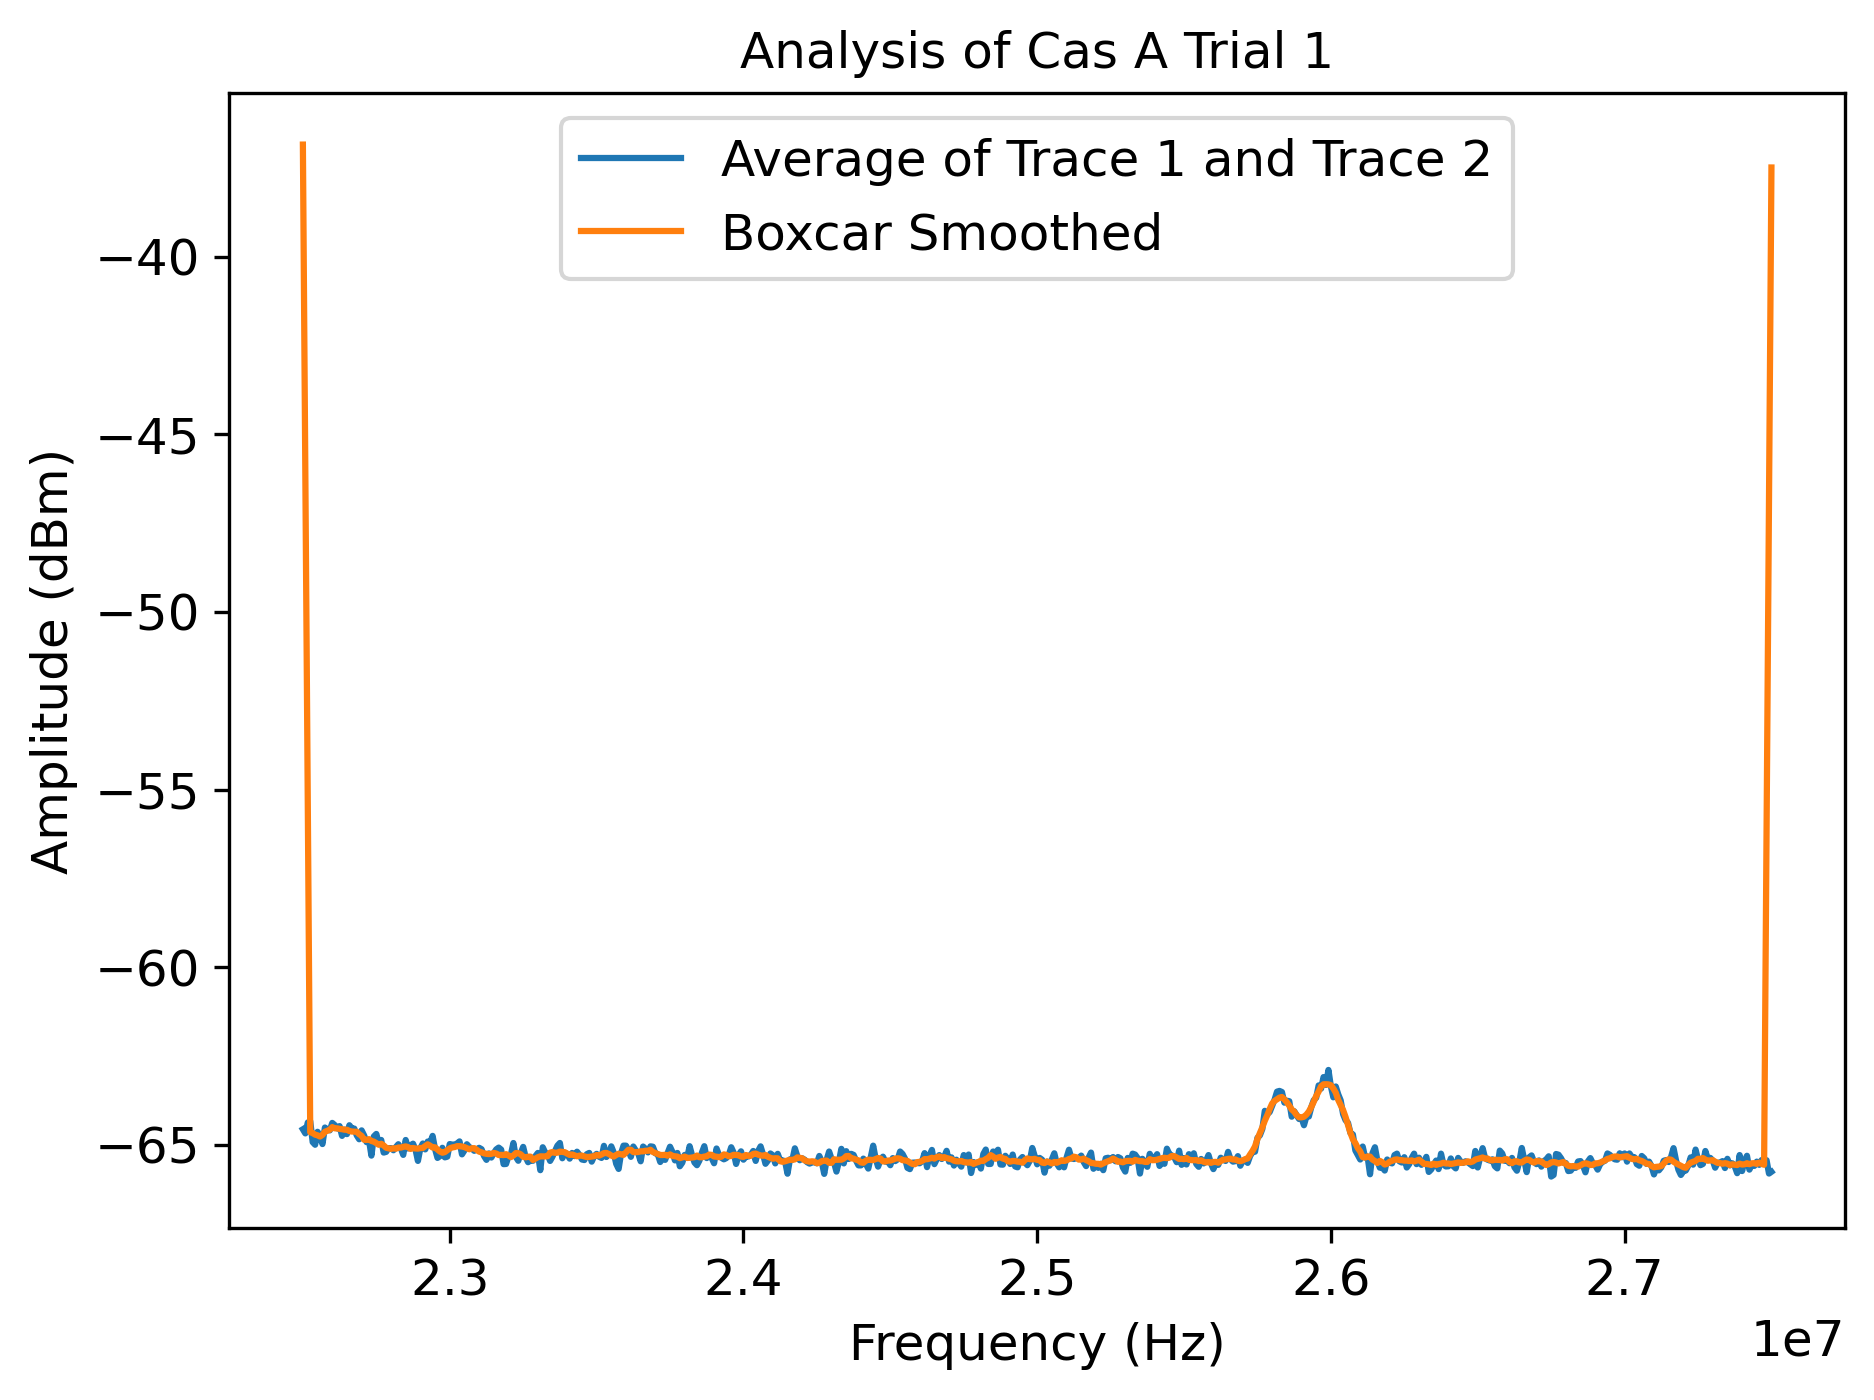
\includegraphics[width=0.85\textwidth]{CasA1_boxcar.png}
\end{center}
\caption{Averaged and smoothed signal for the first Cas A data set}
\label{fig:casa_analysis}
\end{figure}

\begin{figure}[h!]
\begin{center}
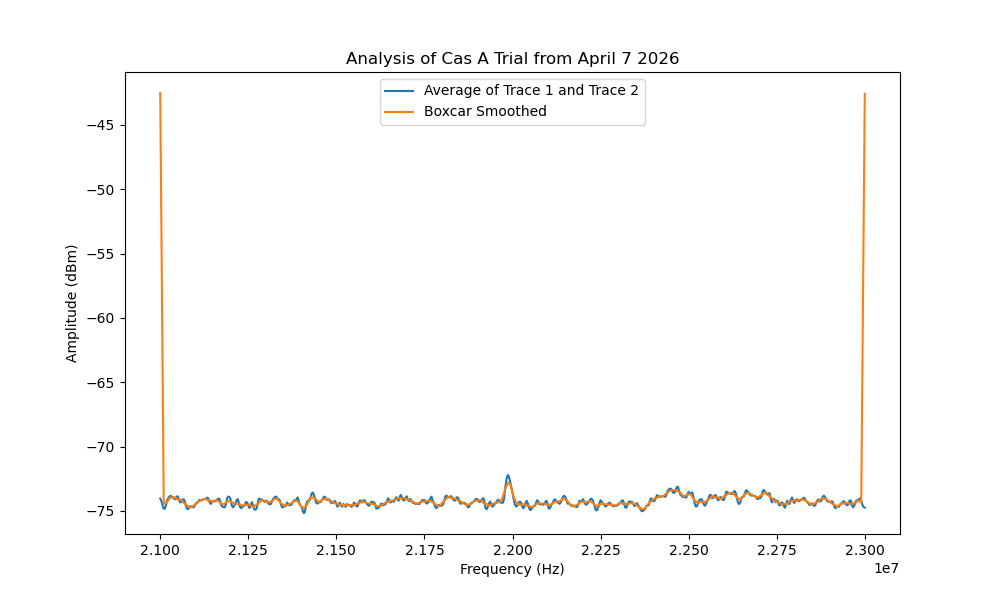
\includegraphics[width=0.85\textwidth]{CasA_040726_boxcar.png}
\end{center}
\caption{Averaged and smoothed signal for the Cas A data collected on April 7 2026}
\label{fig:casa0407_analysis}
\end{figure}

\subsection{Virgo A}

This is the virgo A data set with averaging and smoothing applied

\begin{figure}[h!]
\begin{center}
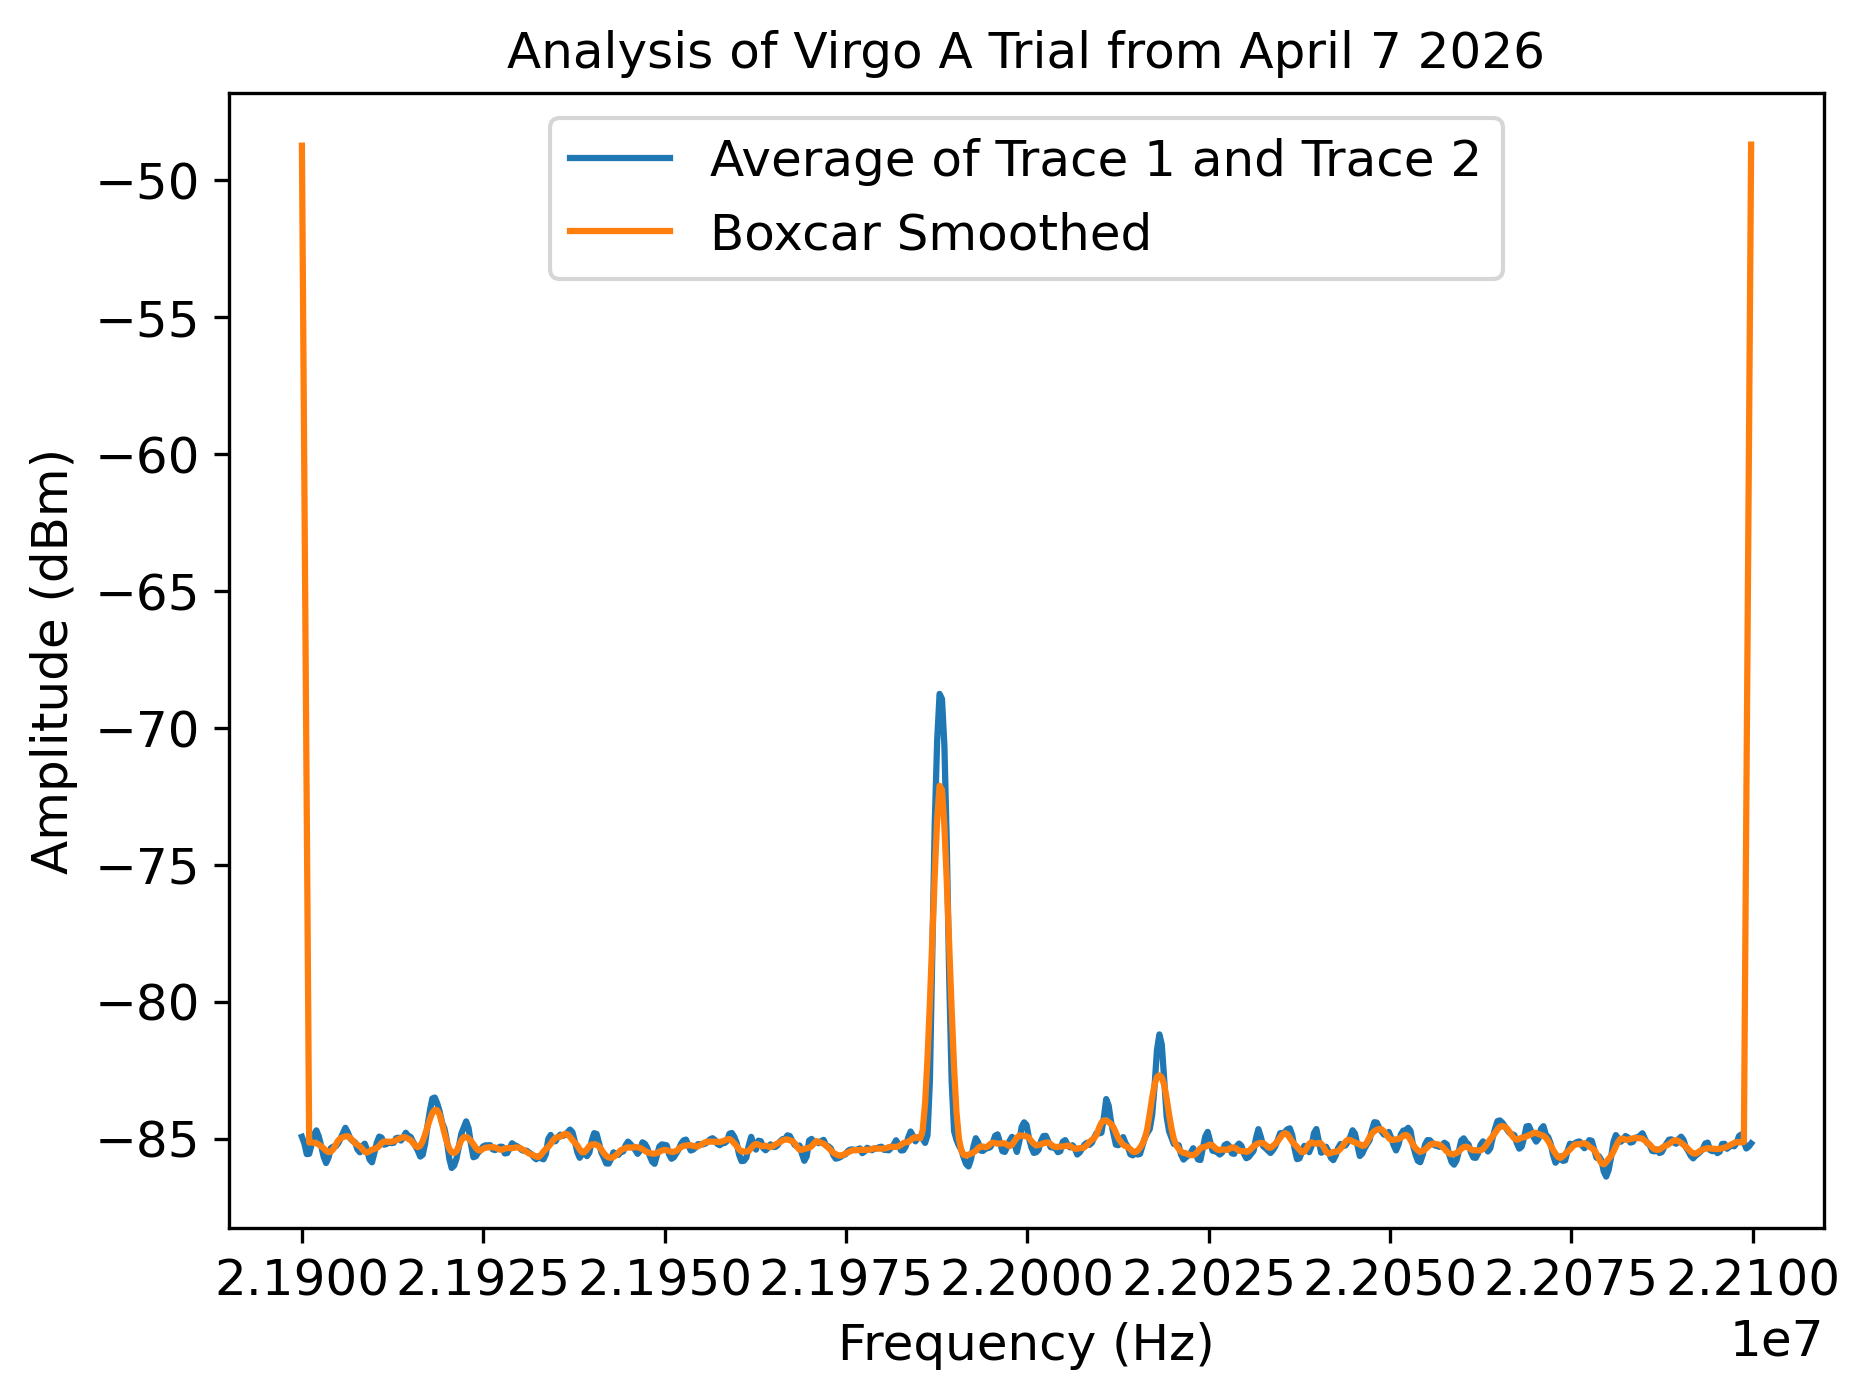
\includegraphics[width=0.85\textwidth]{VirgoA_Boxcar.png}
\end{center}
\caption{Averaged and smoothed signal for the Virgo A data set collected on April 7 2026}
\label{fig:virgoa_analysis}
\end{figure}

